\documentclass[twoside]{book}

% Packages required by doxygen
\usepackage{calc}
\usepackage{doxygen}
\usepackage{graphicx}
\usepackage[utf8]{inputenc}
\usepackage{makeidx}
\usepackage{multicol}
\usepackage{multirow}
\usepackage{textcomp}
\usepackage[table]{xcolor}

% Font selection
\usepackage[T1]{fontenc}
\usepackage{mathptmx}
\usepackage[scaled=.90]{helvet}
\usepackage{courier}
\usepackage{amssymb}
\usepackage{sectsty}
\renewcommand{\familydefault}{\sfdefault}
\allsectionsfont{%
  \fontseries{bc}\selectfont%
  \color{darkgray}%
}
\renewcommand{\DoxyLabelFont}{%
  \fontseries{bc}\selectfont%
  \color{darkgray}%
}

% Page & text layout
\usepackage{geometry}
\geometry{%
  a4paper,%
  top=2.5cm,%
  bottom=2.5cm,%
  left=2.5cm,%
  right=2.5cm%
}
\tolerance=750
\hfuzz=15pt
\hbadness=750
\setlength{\emergencystretch}{15pt}
\setlength{\parindent}{0cm}
\setlength{\parskip}{0.2cm}
\makeatletter
\renewcommand{\paragraph}{%
  \@startsection{paragraph}{4}{0ex}{-1.0ex}{1.0ex}{%
    \normalfont\normalsize\bfseries\SS@parafont%
  }%
}
\renewcommand{\subparagraph}{%
  \@startsection{subparagraph}{5}{0ex}{-1.0ex}{1.0ex}{%
    \normalfont\normalsize\bfseries\SS@subparafont%
  }%
}
\makeatother

% Headers & footers
\usepackage{fancyhdr}
\pagestyle{fancyplain}
\fancyhead[LE]{\fancyplain{}{\bfseries\thepage}}
\fancyhead[CE]{\fancyplain{}{}}
\fancyhead[RE]{\fancyplain{}{\bfseries\leftmark}}
\fancyhead[LO]{\fancyplain{}{\bfseries\rightmark}}
\fancyhead[CO]{\fancyplain{}{}}
\fancyhead[RO]{\fancyplain{}{\bfseries\thepage}}
\fancyfoot[LE]{\fancyplain{}{}}
\fancyfoot[CE]{\fancyplain{}{}}
\fancyfoot[RE]{\fancyplain{}{\bfseries\scriptsize Generated on Sun Oct 20 2013 14\-:25\-:20 for S\-E2\-P by Doxygen }}
\fancyfoot[LO]{\fancyplain{}{\bfseries\scriptsize Generated on Sun Oct 20 2013 14\-:25\-:20 for S\-E2\-P by Doxygen }}
\fancyfoot[CO]{\fancyplain{}{}}
\fancyfoot[RO]{\fancyplain{}{}}
\renewcommand{\footrulewidth}{0.4pt}
\renewcommand{\chaptermark}[1]{%
  \markboth{#1}{}%
}
\renewcommand{\sectionmark}[1]{%
  \markright{\thesection\ #1}%
}

% Indices & bibliography
\usepackage{natbib}
\usepackage[titles]{tocloft}
\setcounter{tocdepth}{3}
\setcounter{secnumdepth}{5}
\makeindex

% Hyperlinks (required, but should be loaded last)
\usepackage{ifpdf}
\ifpdf
  \usepackage[pdftex,pagebackref=true]{hyperref}
\else
  \usepackage[ps2pdf,pagebackref=true]{hyperref}
\fi
\hypersetup{%
  colorlinks=true,%
  linkcolor=blue,%
  citecolor=blue,%
  unicode%
}

% Custom commands
\newcommand{\clearemptydoublepage}{%
  \newpage{\pagestyle{empty}\cleardoublepage}%
}


%===== C O N T E N T S =====

\begin{document}

% Titlepage & ToC
\hypersetup{pageanchor=false}
\pagenumbering{roman}
\begin{titlepage}
\vspace*{7cm}
\begin{center}%
{\Large S\-E2\-P }\\
\vspace*{1cm}
{\large Generated by Doxygen 1.8.5}\\
\vspace*{0.5cm}
{\small Sun Oct 20 2013 14:25:20}\\
\end{center}
\end{titlepage}
\clearemptydoublepage
\tableofcontents
\clearemptydoublepage
\pagenumbering{arabic}
\hypersetup{pageanchor=true}

%--- Begin generated contents ---
\chapter{Namespace Index}
\section{Namespace List}
Here is a list of all documented namespaces with brief descriptions\-:\begin{DoxyCompactList}
\item\contentsline{section}{\hyperlink{namespacethread}{thread} }{\pageref{namespacethread}}{}
\end{DoxyCompactList}

\chapter{Hierarchical Index}
\section{Class Hierarchy}
This inheritance list is sorted roughly, but not completely, alphabetically\-:\begin{DoxyCompactList}
\item \contentsline{section}{Conveyor}{\pageref{classConveyor}}{}
\item \contentsline{section}{Gate}{\pageref{classGate}}{}
\item \contentsline{section}{thread\-:\-:H\-A\-W\-Thread}{\pageref{classthread_1_1HAWThread}}{}
\begin{DoxyCompactList}
\item \contentsline{section}{thread\-:\-:My\-Thread}{\pageref{classthread_1_1MyThread}}{}
\end{DoxyCompactList}
\item \contentsline{section}{Led}{\pageref{classLed}}{}
\item \contentsline{section}{Mutex}{\pageref{classMutex}}{}
\item \contentsline{section}{Serial}{\pageref{classSerial}}{}
\item \contentsline{section}{Traffic\-Light}{\pageref{classTrafficLight}}{}
\end{DoxyCompactList}

\chapter{Class Index}
\section{Class List}
Here are the classes, structs, unions and interfaces with brief descriptions\-:\begin{DoxyCompactList}
\item\contentsline{section}{\hyperlink{classConveyor}{Conveyor} }{\pageref{classConveyor}}{}
\item\contentsline{section}{\hyperlink{classGate}{Gate} }{\pageref{classGate}}{}
\item\contentsline{section}{\hyperlink{classthread_1_1HAWThread}{thread\-::\-H\-A\-W\-Thread} }{\pageref{classthread_1_1HAWThread}}{}
\item\contentsline{section}{\hyperlink{classLed}{Led} }{\pageref{classLed}}{}
\item\contentsline{section}{\hyperlink{classMutex}{Mutex} }{\pageref{classMutex}}{}
\item\contentsline{section}{\hyperlink{classthread_1_1MyThread}{thread\-::\-My\-Thread} }{\pageref{classthread_1_1MyThread}}{}
\item\contentsline{section}{\hyperlink{classSerial}{Serial} }{\pageref{classSerial}}{}
\item\contentsline{section}{\hyperlink{classTrafficLight}{Traffic\-Light} }{\pageref{classTrafficLight}}{}
\end{DoxyCompactList}

\chapter{Namespace Documentation}
\hypertarget{namespacethread}{\section{thread Namespace Reference}
\label{namespacethread}\index{thread@{thread}}
}
\subsection*{Classes}
\begin{DoxyCompactItemize}
\item 
class \hyperlink{classthread_1_1HAWThread}{H\-A\-W\-Thread}
\item 
class \hyperlink{classthread_1_1MyThread}{My\-Thread}
\end{DoxyCompactItemize}


\subsection{Detailed Description}
\hyperlink{classthread_1_1HAWThread}{H\-A\-W\-Thread} class. Encapsulates the most important features of a thread. This serves as a basis for further development. For example, priorities could be passed as constructor argument. 
\chapter{Class Documentation}
\hypertarget{classConveyor}{\section{Conveyor Class Reference}
\label{classConveyor}\index{Conveyor@{Conveyor}}
}
\subsection*{Public Member Functions}
\begin{DoxyCompactItemize}
\item 
\hypertarget{classConveyor_a66b286ad2eee002c8c90f762c4b5aac3}{int {\bfseries get\-Direction} ()}\label{classConveyor_a66b286ad2eee002c8c90f762c4b5aac3}

\item 
\hypertarget{classConveyor_ae1e768294bc1ea396b0cebc8370ca974}{int {\bfseries get\-Speed} ()}\label{classConveyor_ae1e768294bc1ea396b0cebc8370ca974}

\item 
\hypertarget{classConveyor_a95c2fc53e084fac45a2413c772e71f60}{void {\bfseries move\-Right} ()}\label{classConveyor_a95c2fc53e084fac45a2413c772e71f60}

\item 
\hypertarget{classConveyor_a56974e04b8a8e5e760cf59f138888186}{void {\bfseries move\-Left} ()}\label{classConveyor_a56974e04b8a8e5e760cf59f138888186}

\item 
\hypertarget{classConveyor_a9623a77db4c6f9f05455984c9ad41cdf}{void {\bfseries move\-Slow} ()}\label{classConveyor_a9623a77db4c6f9f05455984c9ad41cdf}

\item 
\hypertarget{classConveyor_a2c340ffa3cad9eefd46599a5bf6e07ba}{void {\bfseries conveyor\-Stop} ()}\label{classConveyor_a2c340ffa3cad9eefd46599a5bf6e07ba}

\item 
\hypertarget{classConveyor_a8e7b841155d2f19b42663454d28e9928}{void {\bfseries conveyor\-Continue} ()}\label{classConveyor_a8e7b841155d2f19b42663454d28e9928}

\end{DoxyCompactItemize}
\subsection*{Static Public Member Functions}
\begin{DoxyCompactItemize}
\item 
\hypertarget{classConveyor_a803ec148c4cbb9b9131b67a10d4a5f7f}{static \hyperlink{classConveyor}{Conveyor} $\ast$ {\bfseries get\-Instance} ()}\label{classConveyor_a803ec148c4cbb9b9131b67a10d4a5f7f}

\end{DoxyCompactItemize}


The documentation for this class was generated from the following files\-:\begin{DoxyCompactItemize}
\item 
src/hal/Conveyor.\-h\item 
src/hal/Conveyor.\-cpp\end{DoxyCompactItemize}

\hypertarget{classGate}{\section{Gate Class Reference}
\label{classGate}\index{Gate@{Gate}}
}
\subsection*{Public Member Functions}
\begin{DoxyCompactItemize}
\item 
\hypertarget{classGate_a612d63f09ecbc825508af7cf0a9e245b}{int {\bfseries status} ()}\label{classGate_a612d63f09ecbc825508af7cf0a9e245b}

\item 
\hypertarget{classGate_a3733611cc86dfe641915fcbfaf4d41c8}{void {\bfseries close} ()}\label{classGate_a3733611cc86dfe641915fcbfaf4d41c8}

\item 
\hypertarget{classGate_a6b6e01294cd8f5dbb5c93831c5cd3c3f}{void {\bfseries open} ()}\label{classGate_a6b6e01294cd8f5dbb5c93831c5cd3c3f}

\end{DoxyCompactItemize}
\subsection*{Static Public Member Functions}
\begin{DoxyCompactItemize}
\item 
\hypertarget{classGate_ac4ffd53b738c40cd854b2eb0ed7c6d23}{static \hyperlink{classGate}{Gate} $\ast$ {\bfseries get\-Instance} ()}\label{classGate_ac4ffd53b738c40cd854b2eb0ed7c6d23}

\end{DoxyCompactItemize}


The documentation for this class was generated from the following files\-:\begin{DoxyCompactItemize}
\item 
src/hal/Gate.\-h\item 
src/hal/Gate.\-cpp\end{DoxyCompactItemize}

\hypertarget{classthread_1_1HAWThread}{\section{thread\-:\-:H\-A\-W\-Thread Class Reference}
\label{classthread_1_1HAWThread}\index{thread\-::\-H\-A\-W\-Thread@{thread\-::\-H\-A\-W\-Thread}}
}
Inheritance diagram for thread\-:\-:H\-A\-W\-Thread\-:\begin{figure}[H]
\begin{center}
\leavevmode
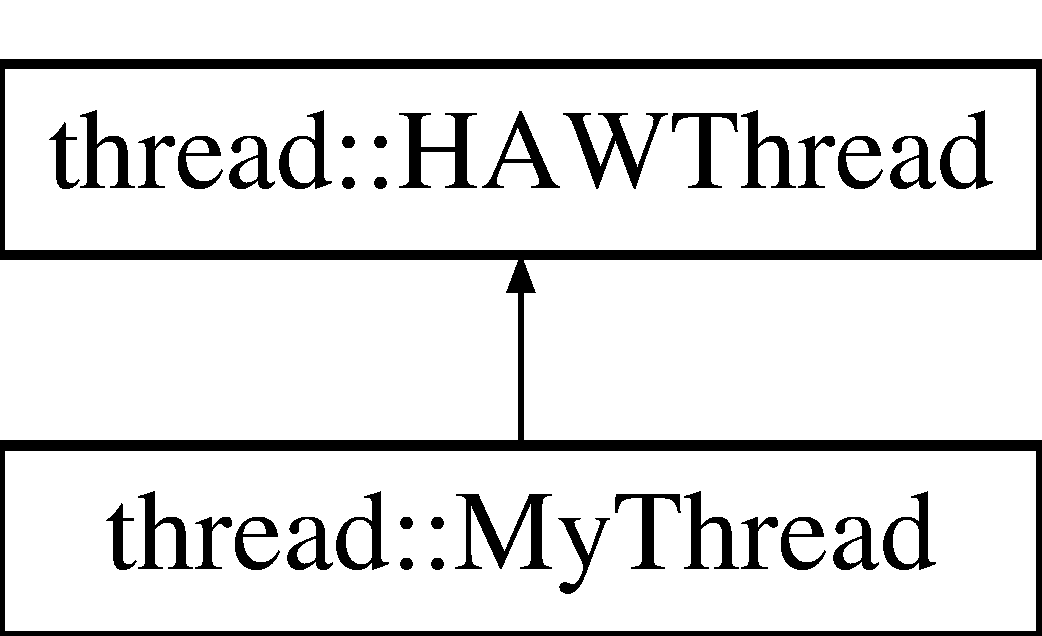
\includegraphics[height=2.000000cm]{classthread_1_1HAWThread}
\end{center}
\end{figure}
\subsection*{Public Member Functions}
\begin{DoxyCompactItemize}
\item 
\hyperlink{classthread_1_1HAWThread_a7ae3280c8aee6ae6536c736a20d92e8d}{H\-A\-W\-Thread} ()
\item 
virtual \hyperlink{classthread_1_1HAWThread_a84706dda23aa384a43ced901381e795b}{$\sim$\-H\-A\-W\-Thread} ()
\item 
void \hyperlink{classthread_1_1HAWThread_ae08d268c337511a1e67fbbeefcb1e89d}{start} (void $\ast$arg)
\item 
void \hyperlink{classthread_1_1HAWThread_ae8a89c83fd7e9b9a712c19f636ab2638}{stop} ()
\item 
void \hyperlink{classthread_1_1HAWThread_a4732efa3445c499f1723971acc07863f}{join} () const 
\item 
void \hyperlink{classthread_1_1HAWThread_a18f2a0cc61833e98b18e56ea541fa38b}{hold} ()
\item 
void \hyperlink{classthread_1_1HAWThread_a4c480261e3236c90c8de73be55650ba4}{cont} ()
\end{DoxyCompactItemize}
\subsection*{Protected Member Functions}
\begin{DoxyCompactItemize}
\item 
void \hyperlink{classthread_1_1HAWThread_a9a3e17be59877d350e310eb19c52679b}{run} (void $\ast$arg)
\item 
virtual void \hyperlink{classthread_1_1HAWThread_ae565cb73c096b246664bd2474b9c8907}{execute} (void $\ast$)=0
\item 
virtual void \hyperlink{classthread_1_1HAWThread_a843ee9493a41cec7e932fdec67a3b244}{shutdown} ()=0
\item 
void $\ast$ \hyperlink{classthread_1_1HAWThread_ab692f3a55b92623653d8213793ba4ebb}{Arg} () const 
\item 
void \hyperlink{classthread_1_1HAWThread_a368c07a801fb8f5e7bb181d2453df4be}{Arg} (void $\ast$a)
\item 
bool \hyperlink{classthread_1_1HAWThread_a46e9f127856f36917b3a8a345b7be5ee}{is\-Stopped} () const 
\item 
void \hyperlink{classthread_1_1HAWThread_a5124385e940aa8d52510a4be10af173c}{shutdown\-All} ()
\end{DoxyCompactItemize}
\subsection*{Static Protected Member Functions}
\begin{DoxyCompactItemize}
\item 
\hypertarget{classthread_1_1HAWThread_a044da2e1a8884a3e2764f9f1863863c7}{static void $\ast$ {\bfseries entry\-Point} (void $\ast$)}\label{classthread_1_1HAWThread_a044da2e1a8884a3e2764f9f1863863c7}

\end{DoxyCompactItemize}


\subsection{Constructor \& Destructor Documentation}
\hypertarget{classthread_1_1HAWThread_a7ae3280c8aee6ae6536c736a20d92e8d}{\index{thread\-::\-H\-A\-W\-Thread@{thread\-::\-H\-A\-W\-Thread}!H\-A\-W\-Thread@{H\-A\-W\-Thread}}
\index{H\-A\-W\-Thread@{H\-A\-W\-Thread}!thread::HAWThread@{thread\-::\-H\-A\-W\-Thread}}
\subsubsection[{H\-A\-W\-Thread}]{\setlength{\rightskip}{0pt plus 5cm}thread\-::\-H\-A\-W\-Thread\-::\-H\-A\-W\-Thread (
\begin{DoxyParamCaption}
{}
\end{DoxyParamCaption}
)}}\label{classthread_1_1HAWThread_a7ae3280c8aee6ae6536c736a20d92e8d}
Constructor. Initializes members \hypertarget{classthread_1_1HAWThread_a84706dda23aa384a43ced901381e795b}{\index{thread\-::\-H\-A\-W\-Thread@{thread\-::\-H\-A\-W\-Thread}!$\sim$\-H\-A\-W\-Thread@{$\sim$\-H\-A\-W\-Thread}}
\index{$\sim$\-H\-A\-W\-Thread@{$\sim$\-H\-A\-W\-Thread}!thread::HAWThread@{thread\-::\-H\-A\-W\-Thread}}
\subsubsection[{$\sim$\-H\-A\-W\-Thread}]{\setlength{\rightskip}{0pt plus 5cm}thread\-::\-H\-A\-W\-Thread\-::$\sim$\-H\-A\-W\-Thread (
\begin{DoxyParamCaption}
{}
\end{DoxyParamCaption}
)\hspace{0.3cm}{\ttfamily [virtual]}}}\label{classthread_1_1HAWThread_a84706dda23aa384a43ced901381e795b}
Destructor. Calls Thread\-Destroy. This should shutdown the thread more carefully. \begin{DoxyWarning}{Warning}
needs some work! 
\end{DoxyWarning}


\subsection{Member Function Documentation}
\hypertarget{classthread_1_1HAWThread_ab692f3a55b92623653d8213793ba4ebb}{\index{thread\-::\-H\-A\-W\-Thread@{thread\-::\-H\-A\-W\-Thread}!Arg@{Arg}}
\index{Arg@{Arg}!thread::HAWThread@{thread\-::\-H\-A\-W\-Thread}}
\subsubsection[{Arg}]{\setlength{\rightskip}{0pt plus 5cm}void$\ast$ thread\-::\-H\-A\-W\-Thread\-::\-Arg (
\begin{DoxyParamCaption}
{}
\end{DoxyParamCaption}
) const\hspace{0.3cm}{\ttfamily [inline]}, {\ttfamily [protected]}}}\label{classthread_1_1HAWThread_ab692f3a55b92623653d8213793ba4ebb}
used internally to pass the argument. \hypertarget{classthread_1_1HAWThread_a368c07a801fb8f5e7bb181d2453df4be}{\index{thread\-::\-H\-A\-W\-Thread@{thread\-::\-H\-A\-W\-Thread}!Arg@{Arg}}
\index{Arg@{Arg}!thread::HAWThread@{thread\-::\-H\-A\-W\-Thread}}
\subsubsection[{Arg}]{\setlength{\rightskip}{0pt plus 5cm}void thread\-::\-H\-A\-W\-Thread\-::\-Arg (
\begin{DoxyParamCaption}
\item[{void $\ast$}]{a}
\end{DoxyParamCaption}
)\hspace{0.3cm}{\ttfamily [inline]}, {\ttfamily [protected]}}}\label{classthread_1_1HAWThread_a368c07a801fb8f5e7bb181d2453df4be}
used internally to set the arguement. \hypertarget{classthread_1_1HAWThread_a4c480261e3236c90c8de73be55650ba4}{\index{thread\-::\-H\-A\-W\-Thread@{thread\-::\-H\-A\-W\-Thread}!cont@{cont}}
\index{cont@{cont}!thread::HAWThread@{thread\-::\-H\-A\-W\-Thread}}
\subsubsection[{cont}]{\setlength{\rightskip}{0pt plus 5cm}void thread\-::\-H\-A\-W\-Thread\-::cont (
\begin{DoxyParamCaption}
{}
\end{DoxyParamCaption}
)}}\label{classthread_1_1HAWThread_a4c480261e3236c90c8de73be55650ba4}
This function continues (resumes) the thread. It makes a Thread\-Ctrl call. \hypertarget{classthread_1_1HAWThread_ae565cb73c096b246664bd2474b9c8907}{\index{thread\-::\-H\-A\-W\-Thread@{thread\-::\-H\-A\-W\-Thread}!execute@{execute}}
\index{execute@{execute}!thread::HAWThread@{thread\-::\-H\-A\-W\-Thread}}
\subsubsection[{execute}]{\setlength{\rightskip}{0pt plus 5cm}virtual void thread\-::\-H\-A\-W\-Thread\-::execute (
\begin{DoxyParamCaption}
\item[{void $\ast$}]{}
\end{DoxyParamCaption}
)\hspace{0.3cm}{\ttfamily [protected]}, {\ttfamily [pure virtual]}}}\label{classthread_1_1HAWThread_ae565cb73c096b246664bd2474b9c8907}
to be implemented in the derived class. The application programmer has to write his own loop. He can check bool \hyperlink{classthread_1_1HAWThread_a46e9f127856f36917b3a8a345b7be5ee}{is\-Stopped()} to see if the thread should exit the loop. 

Implemented in \hyperlink{classthread_1_1MyThread_a434a2bc9bc3e89e9bc87a638e18be6ee}{thread\-::\-My\-Thread}.

\hypertarget{classthread_1_1HAWThread_a18f2a0cc61833e98b18e56ea541fa38b}{\index{thread\-::\-H\-A\-W\-Thread@{thread\-::\-H\-A\-W\-Thread}!hold@{hold}}
\index{hold@{hold}!thread::HAWThread@{thread\-::\-H\-A\-W\-Thread}}
\subsubsection[{hold}]{\setlength{\rightskip}{0pt plus 5cm}void thread\-::\-H\-A\-W\-Thread\-::hold (
\begin{DoxyParamCaption}
{}
\end{DoxyParamCaption}
)}}\label{classthread_1_1HAWThread_a18f2a0cc61833e98b18e56ea541fa38b}
This function holds (suspends) the thread. It makes a Thread\-Ctrl call. It shall be used if the thread is not being used for a while but may be used later \hypertarget{classthread_1_1HAWThread_a46e9f127856f36917b3a8a345b7be5ee}{\index{thread\-::\-H\-A\-W\-Thread@{thread\-::\-H\-A\-W\-Thread}!is\-Stopped@{is\-Stopped}}
\index{is\-Stopped@{is\-Stopped}!thread::HAWThread@{thread\-::\-H\-A\-W\-Thread}}
\subsubsection[{is\-Stopped}]{\setlength{\rightskip}{0pt plus 5cm}bool thread\-::\-H\-A\-W\-Thread\-::is\-Stopped (
\begin{DoxyParamCaption}
{}
\end{DoxyParamCaption}
) const\hspace{0.3cm}{\ttfamily [inline]}, {\ttfamily [protected]}}}\label{classthread_1_1HAWThread_a46e9f127856f36917b3a8a345b7be5ee}
returns the stop-\/status of the thread. This function should be checked by the user function execute regularly. \hypertarget{classthread_1_1HAWThread_a4732efa3445c499f1723971acc07863f}{\index{thread\-::\-H\-A\-W\-Thread@{thread\-::\-H\-A\-W\-Thread}!join@{join}}
\index{join@{join}!thread::HAWThread@{thread\-::\-H\-A\-W\-Thread}}
\subsubsection[{join}]{\setlength{\rightskip}{0pt plus 5cm}void thread\-::\-H\-A\-W\-Thread\-::join (
\begin{DoxyParamCaption}
{}
\end{DoxyParamCaption}
) const}}\label{classthread_1_1HAWThread_a4732efa3445c499f1723971acc07863f}
Calls join on the thread. \begin{DoxyWarning}{Warning}
must be called from the same context as start. 
\end{DoxyWarning}
\hypertarget{classthread_1_1HAWThread_a9a3e17be59877d350e310eb19c52679b}{\index{thread\-::\-H\-A\-W\-Thread@{thread\-::\-H\-A\-W\-Thread}!run@{run}}
\index{run@{run}!thread::HAWThread@{thread\-::\-H\-A\-W\-Thread}}
\subsubsection[{run}]{\setlength{\rightskip}{0pt plus 5cm}void thread\-::\-H\-A\-W\-Thread\-::run (
\begin{DoxyParamCaption}
\item[{void $\ast$}]{arg}
\end{DoxyParamCaption}
)\hspace{0.3cm}{\ttfamily [protected]}}}\label{classthread_1_1HAWThread_a9a3e17be59877d350e310eb19c52679b}
This is called when the thread is started. It calls execute an shutdown which are the user functions. \hypertarget{classthread_1_1HAWThread_a843ee9493a41cec7e932fdec67a3b244}{\index{thread\-::\-H\-A\-W\-Thread@{thread\-::\-H\-A\-W\-Thread}!shutdown@{shutdown}}
\index{shutdown@{shutdown}!thread::HAWThread@{thread\-::\-H\-A\-W\-Thread}}
\subsubsection[{shutdown}]{\setlength{\rightskip}{0pt plus 5cm}virtual void thread\-::\-H\-A\-W\-Thread\-::shutdown (
\begin{DoxyParamCaption}
{}
\end{DoxyParamCaption}
)\hspace{0.3cm}{\ttfamily [protected]}, {\ttfamily [pure virtual]}}}\label{classthread_1_1HAWThread_a843ee9493a41cec7e932fdec67a3b244}
this function must be implemented in the derived class. The function is called once after the thread has been stopped. 

Implemented in \hyperlink{classthread_1_1MyThread_a8d381c9d7c7690f379ad7992c0dcc5a2}{thread\-::\-My\-Thread}.

\hypertarget{classthread_1_1HAWThread_a5124385e940aa8d52510a4be10af173c}{\index{thread\-::\-H\-A\-W\-Thread@{thread\-::\-H\-A\-W\-Thread}!shutdown\-All@{shutdown\-All}}
\index{shutdown\-All@{shutdown\-All}!thread::HAWThread@{thread\-::\-H\-A\-W\-Thread}}
\subsubsection[{shutdown\-All}]{\setlength{\rightskip}{0pt plus 5cm}void thread\-::\-H\-A\-W\-Thread\-::shutdown\-All (
\begin{DoxyParamCaption}
{}
\end{DoxyParamCaption}
)\hspace{0.3cm}{\ttfamily [inline]}, {\ttfamily [protected]}}}\label{classthread_1_1HAWThread_a5124385e940aa8d52510a4be10af173c}
sets the G\-L\-O\-B\-A\-L\-\_\-\-E\-X\-I\-T flag to true. \hypertarget{classthread_1_1HAWThread_ae08d268c337511a1e67fbbeefcb1e89d}{\index{thread\-::\-H\-A\-W\-Thread@{thread\-::\-H\-A\-W\-Thread}!start@{start}}
\index{start@{start}!thread::HAWThread@{thread\-::\-H\-A\-W\-Thread}}
\subsubsection[{start}]{\setlength{\rightskip}{0pt plus 5cm}void thread\-::\-H\-A\-W\-Thread\-::start (
\begin{DoxyParamCaption}
\item[{void $\ast$}]{arg}
\end{DoxyParamCaption}
)}}\label{classthread_1_1HAWThread_ae08d268c337511a1e67fbbeefcb1e89d}
Starts the Thread. \begin{DoxyWarning}{Warning}
start must be called always from the same context as \hyperlink{classthread_1_1HAWThread_ae8a89c83fd7e9b9a712c19f636ab2638}{stop()}. 

If Thread is already running, \hyperlink{classthread_1_1HAWThread_ae08d268c337511a1e67fbbeefcb1e89d}{start()} is a N\-O\-P. \begin{DoxyItemize}
\item argument is stored locally as a member. \end{DoxyItemize}

\end{DoxyWarning}
\hypertarget{classthread_1_1HAWThread_ae8a89c83fd7e9b9a712c19f636ab2638}{\index{thread\-::\-H\-A\-W\-Thread@{thread\-::\-H\-A\-W\-Thread}!stop@{stop}}
\index{stop@{stop}!thread::HAWThread@{thread\-::\-H\-A\-W\-Thread}}
\subsubsection[{stop}]{\setlength{\rightskip}{0pt plus 5cm}void thread\-::\-H\-A\-W\-Thread\-::stop (
\begin{DoxyParamCaption}
{}
\end{DoxyParamCaption}
)}}\label{classthread_1_1HAWThread_ae8a89c83fd7e9b9a712c19f636ab2638}
Sets the internal flag L\-O\-C\-A\-L\-\_\-\-E\-X\-I\-T to true. 

The documentation for this class was generated from the following files\-:\begin{DoxyCompactItemize}
\item 
src/H\-A\-W\-Thread.\-h\item 
src/H\-A\-W\-Thread.\-cpp\end{DoxyCompactItemize}

\hypertarget{classLed}{\section{Led Class Reference}
\label{classLed}\index{Led@{Led}}
}
\subsection*{Public Member Functions}
\begin{DoxyCompactItemize}
\item 
\hypertarget{classLed_ae975e138319b442936117fba1ec3a618}{void {\bfseries led\-\_\-\-Start\-Button\-\_\-\-On} ()}\label{classLed_ae975e138319b442936117fba1ec3a618}

\item 
\hypertarget{classLed_af7dc6d8a2760d1dbe61f5219d72a9613}{void {\bfseries led\-\_\-\-Start\-Button\-\_\-\-Off} ()}\label{classLed_af7dc6d8a2760d1dbe61f5219d72a9613}

\item 
\hypertarget{classLed_a4f13d40b3e284aae8679b584f223db29}{void {\bfseries led\-\_\-\-Reset\-Button\-\_\-\-On} ()}\label{classLed_a4f13d40b3e284aae8679b584f223db29}

\item 
\hypertarget{classLed_a153abe5004c72fc1bede1035e3615c56}{void {\bfseries led\-\_\-\-Reset\-Button\-\_\-\-Off} ()}\label{classLed_a153abe5004c72fc1bede1035e3615c56}

\item 
\hypertarget{classLed_a8d188ba11a0c97cc01389a83d66003a5}{void {\bfseries led\-\_\-\-Q1\-\_\-\-On} ()}\label{classLed_a8d188ba11a0c97cc01389a83d66003a5}

\item 
\hypertarget{classLed_a49f3d340c9ce2ca8edc1483678c2ef97}{void {\bfseries led\-\_\-\-Q1\-\_\-\-Off} ()}\label{classLed_a49f3d340c9ce2ca8edc1483678c2ef97}

\item 
\hypertarget{classLed_a9dbd288be5f39d9b7f01c873593d4f1f}{void {\bfseries led\-\_\-\-Q2\-\_\-\-On} ()}\label{classLed_a9dbd288be5f39d9b7f01c873593d4f1f}

\item 
\hypertarget{classLed_a75b30e02b600f8c2237053f86fe17da7}{void {\bfseries led\-\_\-\-Q2\-\_\-\-Off} ()}\label{classLed_a75b30e02b600f8c2237053f86fe17da7}

\end{DoxyCompactItemize}
\subsection*{Static Public Member Functions}
\begin{DoxyCompactItemize}
\item 
\hypertarget{classLed_ab7c85469a3885c9ec891daca461f3a16}{static \hyperlink{classLed}{Led} $\ast$ {\bfseries get\-Instance} ()}\label{classLed_ab7c85469a3885c9ec891daca461f3a16}

\end{DoxyCompactItemize}


The documentation for this class was generated from the following files\-:\begin{DoxyCompactItemize}
\item 
src/hal/Led.\-h\item 
src/hal/Led.\-cpp\end{DoxyCompactItemize}

\hypertarget{classMutex}{\section{Mutex Class Reference}
\label{classMutex}\index{Mutex@{Mutex}}
}
\subsection*{Public Member Functions}
\begin{DoxyCompactItemize}
\item 
\hypertarget{classMutex_a593423d868daf926c7b0d63a833ae29a}{\hyperlink{classMutex_a593423d868daf926c7b0d63a833ae29a}{Mutex} ()}\label{classMutex_a593423d868daf926c7b0d63a833ae29a}

\begin{DoxyCompactList}\small\item\em mutex-\/constructor \end{DoxyCompactList}\item 
\hypertarget{classMutex_ac9e9182407f5f74892318607888e9be4}{virtual \hyperlink{classMutex_ac9e9182407f5f74892318607888e9be4}{$\sim$\-Mutex} ()}\label{classMutex_ac9e9182407f5f74892318607888e9be4}

\begin{DoxyCompactList}\small\item\em mutex-\/deconstructor \end{DoxyCompactList}\item 
\hypertarget{classMutex_ad91be808bf0a60a16f10b897ec246d3a}{void \hyperlink{classMutex_ad91be808bf0a60a16f10b897ec246d3a}{lock} ()}\label{classMutex_ad91be808bf0a60a16f10b897ec246d3a}

\begin{DoxyCompactList}\small\item\em locks the mutex \end{DoxyCompactList}\item 
\hypertarget{classMutex_a546a5b797ba29959357586aa2b3740a8}{void \hyperlink{classMutex_a546a5b797ba29959357586aa2b3740a8}{unlock} ()}\label{classMutex_a546a5b797ba29959357586aa2b3740a8}

\begin{DoxyCompactList}\small\item\em unlocks the mutex \end{DoxyCompactList}\end{DoxyCompactItemize}


The documentation for this class was generated from the following files\-:\begin{DoxyCompactItemize}
\item 
src/Mutex.\-h\item 
src/Mutex.\-cpp\end{DoxyCompactItemize}

\hypertarget{classthread_1_1MyThread}{\section{thread\-:\-:My\-Thread Class Reference}
\label{classthread_1_1MyThread}\index{thread\-::\-My\-Thread@{thread\-::\-My\-Thread}}
}
Inheritance diagram for thread\-:\-:My\-Thread\-:\begin{figure}[H]
\begin{center}
\leavevmode
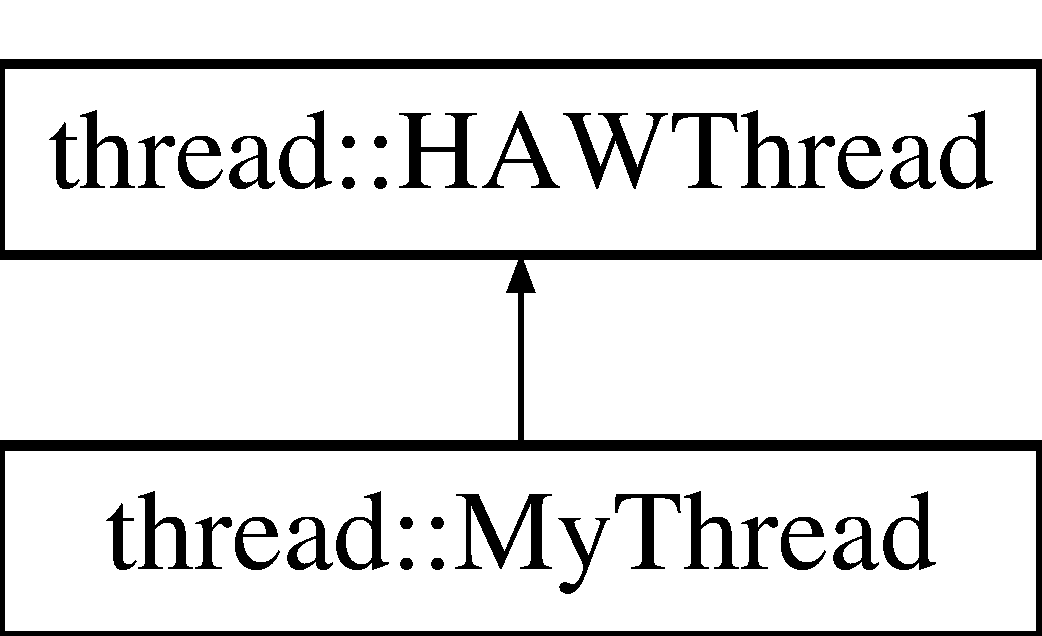
\includegraphics[height=2.000000cm]{classthread_1_1MyThread}
\end{center}
\end{figure}
\subsection*{Public Member Functions}
\begin{DoxyCompactItemize}
\item 
virtual void \hyperlink{classthread_1_1MyThread_a434a2bc9bc3e89e9bc87a638e18be6ee}{execute} (void $\ast$arg)
\item 
virtual void \hyperlink{classthread_1_1MyThread_a8d381c9d7c7690f379ad7992c0dcc5a2}{shutdown} ()
\end{DoxyCompactItemize}
\subsection*{Additional Inherited Members}


\subsection{Member Function Documentation}
\hypertarget{classthread_1_1MyThread_a434a2bc9bc3e89e9bc87a638e18be6ee}{\index{thread\-::\-My\-Thread@{thread\-::\-My\-Thread}!execute@{execute}}
\index{execute@{execute}!thread::MyThread@{thread\-::\-My\-Thread}}
\subsubsection[{execute}]{\setlength{\rightskip}{0pt plus 5cm}void thread\-::\-My\-Thread\-::execute (
\begin{DoxyParamCaption}
\item[{void $\ast$}]{}
\end{DoxyParamCaption}
)\hspace{0.3cm}{\ttfamily [virtual]}}}\label{classthread_1_1MyThread_a434a2bc9bc3e89e9bc87a638e18be6ee}
to be implemented in the derived class. The application programmer has to write his own loop. He can check bool \hyperlink{classthread_1_1HAWThread_a46e9f127856f36917b3a8a345b7be5ee}{is\-Stopped()} to see if the thread should exit the loop. 

Implements \hyperlink{classthread_1_1HAWThread_ae565cb73c096b246664bd2474b9c8907}{thread\-::\-H\-A\-W\-Thread}.

\hypertarget{classthread_1_1MyThread_a8d381c9d7c7690f379ad7992c0dcc5a2}{\index{thread\-::\-My\-Thread@{thread\-::\-My\-Thread}!shutdown@{shutdown}}
\index{shutdown@{shutdown}!thread::MyThread@{thread\-::\-My\-Thread}}
\subsubsection[{shutdown}]{\setlength{\rightskip}{0pt plus 5cm}void thread\-::\-My\-Thread\-::shutdown (
\begin{DoxyParamCaption}
{}
\end{DoxyParamCaption}
)\hspace{0.3cm}{\ttfamily [virtual]}}}\label{classthread_1_1MyThread_a8d381c9d7c7690f379ad7992c0dcc5a2}
this function must be implemented in the derived class. The function is called once after the thread has been stopped. 

Implements \hyperlink{classthread_1_1HAWThread_a843ee9493a41cec7e932fdec67a3b244}{thread\-::\-H\-A\-W\-Thread}.



The documentation for this class was generated from the following files\-:\begin{DoxyCompactItemize}
\item 
src/milestone1/My\-Thread.\-h\item 
src/milestone1/My\-Thread.\-cpp\end{DoxyCompactItemize}

\hypertarget{classSerial}{\section{Serial Class Reference}
\label{classSerial}\index{Serial@{Serial}}
}
\subsection*{Public Member Functions}
\begin{DoxyCompactItemize}
\item 
\hypertarget{classSerial_a169ed0c2a5bccec7857ab501aaf35b87}{int {\bfseries send\-Message} (char message)}\label{classSerial_a169ed0c2a5bccec7857ab501aaf35b87}

\item 
\hypertarget{classSerial_a56af97dad1a41aa3a12de86209f1c1e3}{int {\bfseries read\-Message} (char $\ast$buffer)}\label{classSerial_a56af97dad1a41aa3a12de86209f1c1e3}

\end{DoxyCompactItemize}


The documentation for this class was generated from the following files\-:\begin{DoxyCompactItemize}
\item 
src/hal/Serial.\-h\item 
src/hal/Serial.\-cpp\end{DoxyCompactItemize}

\hypertarget{classTrafficLight}{\section{Traffic\-Light Class Reference}
\label{classTrafficLight}\index{Traffic\-Light@{Traffic\-Light}}
}
\subsection*{Public Member Functions}
\begin{DoxyCompactItemize}
\item 
\hypertarget{classTrafficLight_abe5851461f1a78fcdaf845eccb3815cb}{int {\bfseries status\-Red} ()}\label{classTrafficLight_abe5851461f1a78fcdaf845eccb3815cb}

\item 
\hypertarget{classTrafficLight_a70be96340b4b25d3a638e5f290606887}{int {\bfseries status\-Yellow} ()}\label{classTrafficLight_a70be96340b4b25d3a638e5f290606887}

\item 
\hypertarget{classTrafficLight_a6abb2ec2fc47d8ef7abc38cd7e1ce1e4}{int {\bfseries status\-Green} ()}\label{classTrafficLight_a6abb2ec2fc47d8ef7abc38cd7e1ce1e4}

\item 
\hypertarget{classTrafficLight_a2cb443a633011acc36f147bfb96a01c8}{void {\bfseries red\-On} ()}\label{classTrafficLight_a2cb443a633011acc36f147bfb96a01c8}

\item 
\hypertarget{classTrafficLight_acef2029900662056507e42ffebef6df3}{void {\bfseries red\-Off} ()}\label{classTrafficLight_acef2029900662056507e42ffebef6df3}

\item 
\hypertarget{classTrafficLight_a1d97dcc2d58b2c0f08fab2eb2b902b32}{void {\bfseries yellow\-On} ()}\label{classTrafficLight_a1d97dcc2d58b2c0f08fab2eb2b902b32}

\item 
\hypertarget{classTrafficLight_a215cb8496fb1f3c05a0d88becc196cd9}{void {\bfseries yellow\-Off} ()}\label{classTrafficLight_a215cb8496fb1f3c05a0d88becc196cd9}

\item 
\hypertarget{classTrafficLight_a54e92a2b3dfb4fa8232b98d045615440}{void {\bfseries green\-On} ()}\label{classTrafficLight_a54e92a2b3dfb4fa8232b98d045615440}

\item 
\hypertarget{classTrafficLight_ae0742cdeaabe4a54edc4b69647f7f59e}{void {\bfseries green\-Off} ()}\label{classTrafficLight_ae0742cdeaabe4a54edc4b69647f7f59e}

\end{DoxyCompactItemize}
\subsection*{Static Public Member Functions}
\begin{DoxyCompactItemize}
\item 
\hypertarget{classTrafficLight_aea8fff7123abb6e9935992e60be85780}{static \hyperlink{classTrafficLight}{Traffic\-Light} $\ast$ {\bfseries get\-Instance} ()}\label{classTrafficLight_aea8fff7123abb6e9935992e60be85780}

\end{DoxyCompactItemize}


The documentation for this class was generated from the following files\-:\begin{DoxyCompactItemize}
\item 
src/hal/Traffic\-Light.\-h\item 
src/hal/Traffic\-Light.\-cpp\end{DoxyCompactItemize}

%--- End generated contents ---

% Index
\newpage
\phantomsection
\addcontentsline{toc}{part}{Index}
\printindex

\end{document}
